\begin{figure}
	\centering
    \caption{Uma estrutura discretizada em elementos CST.}
    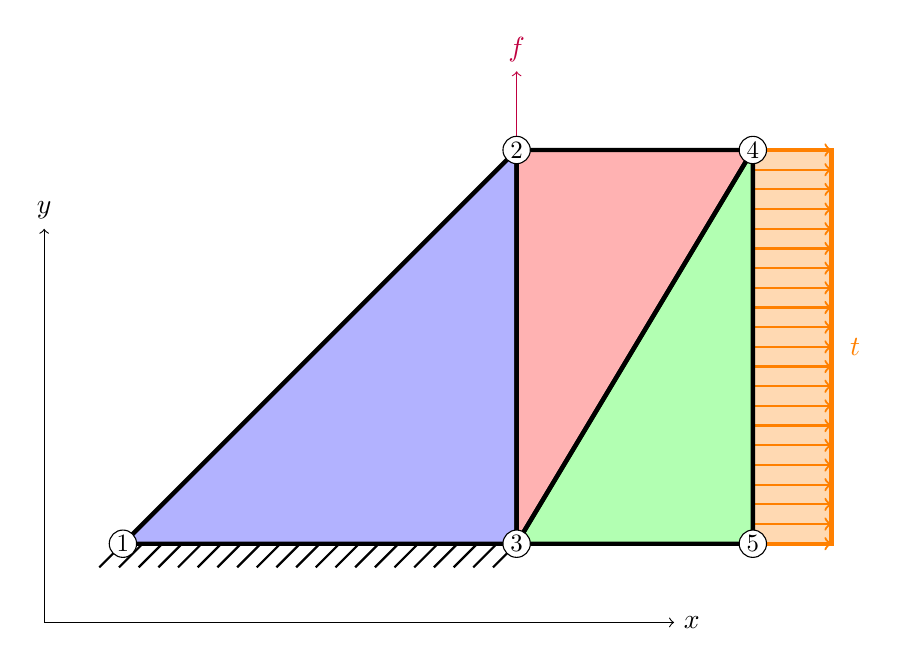
\begin{tikzpicture}
        \usetikzlibrary{calc}
        \coordinate  (1) at (0 cm,0 cm);
        \coordinate  (2) at (5 cm, 5 cm);
        \coordinate  (3) at (5 cm, 0 cm);
        \coordinate  (4) at (8 cm, 5 cm);
        \coordinate  (5) at (8 cm, 0 cm);

        \draw[orange, ultra thick, fill = orange, fill opacity = 0.3] (4) -- (5) --++ (1 cm, 0 cm) --++ (0 cm, 5 cm) -- cycle;

    
                
        \draw[->, orange, thick] (4) ++ ($ 0.0*(5)-0.0*(4)$) --++ (1cm, 0cm);
        \draw[->, orange, thick] (4) ++ ($ 0.05*(5)-0.05*(4)$) --++ (1cm, 0cm);
        \draw[->, orange, thick] (4) ++ ($ 0.1*(5)-0.1*(4)$) --++ (1cm, 0cm);
        \draw[->, orange, thick] (4) ++ ($ 0.15*(5)-0.15*(4)$) --++ (1cm, 0cm);
        \draw[->, orange, thick] (4) ++ ($ 0.2*(5)-0.2*(4)$) --++ (1cm, 0cm);
        \draw[->, orange, thick] (4) ++ ($ 0.25*(5)-0.25*(4)$) --++ (1cm, 0cm);
        \draw[->, orange, thick] (4) ++ ($ 0.3*(5)-0.3*(4)$) --++ (1cm, 0cm);
        \draw[->, orange, thick] (4) ++ ($ 0.35*(5)-0.35*(4)$) --++ (1cm, 0cm);
        \draw[->, orange, thick] (4) ++ ($ 0.4*(5)-0.4*(4)$) --++ (1cm, 0cm);
        \draw[->, orange, thick] (4) ++ ($ 0.45*(5)-0.45*(4)$) --++ (1cm, 0cm);
        \draw[->, orange, thick] (4) ++ ($ 0.5*(5)-0.5*(4)$) --++ (1cm, 0cm);
        \draw[->, orange, thick] (4) ++ ($ 0.55*(5)-0.55*(4)$) --++ (1cm, 0cm);
        \draw[->, orange, thick] (4) ++ ($ 0.6*(5)-0.6*(4)$) --++ (1cm, 0cm);
        \draw[->, orange, thick] (4) ++ ($ 0.65*(5)-0.65*(4)$) --++ (1cm, 0cm);
        \draw[->, orange, thick] (4) ++ ($ 0.7*(5)-0.7*(4)$) --++ (1cm, 0cm);
        \draw[->, orange, thick] (4) ++ ($ 0.75*(5)-0.75*(4)$) --++ (1cm, 0cm);
        \draw[->, orange, thick] (4) ++ ($ 0.8*(5)-0.8*(4)$) --++ (1cm, 0cm);
        \draw[->, orange, thick] (4) ++ ($ 0.85*(5)-0.85*(4)$) --++ (1cm, 0cm);
        \draw[->, orange, thick] (4) ++ ($ 0.9*(5)-0.9*(4)$) --++ (1cm, 0cm);
        \draw[->, orange, thick] (4) ++ ($ 0.95*(5)-0.95*(4)$) --++ (1cm, 0cm);
        \draw[->, orange, thick] (4) ++ ($ 1.0*(5)-1.0*(4)$) --++ (1cm, 0cm);
                    
        \draw[black, ultra thick, fill = blue, fill opacity = 0.3] (1) -- (2) -- (3) -- cycle;
        \draw[black, ultra thick, fill = red, fill opacity = 0.3] (2) -- (3) -- (4) -- cycle;
        \draw[black, ultra thick, fill = green, fill opacity = 0.3] (3) -- (4) -- (5) -- cycle;

        \draw[->, purple] (2) --++(0 cm, 1 cm) node[above, purple]{$f$};

        
        \draw[thick] ($0.0*(3)$) --++ (-0.3 cm, -0.3 cm);
        \draw[thick] ($0.05*(3)$) --++ (-0.3 cm, -0.3 cm);
        \draw[thick] ($0.1*(3)$) --++ (-0.3 cm, -0.3 cm);
        \draw[thick] ($0.15*(3)$) --++ (-0.3 cm, -0.3 cm);
        \draw[thick] ($0.2*(3)$) --++ (-0.3 cm, -0.3 cm);
        \draw[thick] ($0.25*(3)$) --++ (-0.3 cm, -0.3 cm);
        \draw[thick] ($0.3*(3)$) --++ (-0.3 cm, -0.3 cm);
        \draw[thick] ($0.35*(3)$) --++ (-0.3 cm, -0.3 cm);
        \draw[thick] ($0.4*(3)$) --++ (-0.3 cm, -0.3 cm);
        \draw[thick] ($0.45*(3)$) --++ (-0.3 cm, -0.3 cm);
        \draw[thick] ($0.5*(3)$) --++ (-0.3 cm, -0.3 cm);
        \draw[thick] ($0.55*(3)$) --++ (-0.3 cm, -0.3 cm);
        \draw[thick] ($0.6*(3)$) --++ (-0.3 cm, -0.3 cm);
        \draw[thick] ($0.65*(3)$) --++ (-0.3 cm, -0.3 cm);
        \draw[thick] ($0.7*(3)$) --++ (-0.3 cm, -0.3 cm);
        \draw[thick] ($0.75*(3)$) --++ (-0.3 cm, -0.3 cm);
        \draw[thick] ($0.8*(3)$) --++ (-0.3 cm, -0.3 cm);
        \draw[thick] ($0.85*(3)$) --++ (-0.3 cm, -0.3 cm);
        \draw[thick] ($0.9*(3)$) --++ (-0.3 cm, -0.3 cm);
        \draw[thick] ($0.95*(3)$) --++ (-0.3 cm, -0.3 cm);
        \draw[thick] ($1.0*(3)$) --++ (-0.3 cm, -0.3 cm);

        \draw ($0.5*(5) + 0.5*(4)$) ++ (1.3 cm, 0 cm) node[orange] {$t$};

        
        \draw (1) node[circle, draw, inner sep=1pt, fill=white, thin, scale = 0.9, fill opacity = 1] {$1$};
        \draw (2) node[circle, draw, inner sep=1pt, fill=white, thin, scale = 0.9, fill opacity = 1] {$2$};
        \draw (3) node[circle, draw, inner sep=1pt, fill=white, thin, scale = 0.9, fill opacity = 1] {$3$};
        \draw (4) node[circle, draw, inner sep=1pt, fill=white, thin, scale = 0.9, fill opacity = 1] {$4$};
        \draw (5) node[circle, draw, inner sep=1pt, fill=white, thin, scale = 0.9, fill opacity = 1] {$5$};

        \draw[->] (-1 cm, -1 cm) --++ (8 cm, 0 cm) node[right] {$x$};
        \draw[->] (-1 cm, -1 cm) --++ (0 cm, 5 cm) node[above] {$y$};
    \end{tikzpicture}
    \label{fig:exemplo_matriz_global}
    \fonte{\me{2022}}
\end{figure}